\section{Analysis}
\unsure{Equations for all?}
\subsection{Comparing text of the tweet and document}

To determine if the tweets promoting the articles could be generated from the document text, we try and find the degree of common words between the tweet and the text of the document. We also checked least common subsequences between the tweet and the document. These values combined together give a fairly good approximation of the degree to which the tweet is extracted from the document text. For all these analyses, the stop words have been eliminated from the tweet as well as the document, so that only the significant words are taken into consideration. The hastags, references (@) and URLs from the tweets were also all removed.

\subsubsection {Total match with text in article}

To calculate the position of tweet text as a whole in the text, we checked for a complete substring match of the tweet in the text. Out of the 6144 instances where a tweet text was checked against the text in the article, a complete match was found around 70 times\change{recheck these numbers, correct in graph}, as shown in \figref{fig:positions}. 30 times out of these, the tweet text had been matched against the title of the article extracted into the text. The rest of the results are significant, since the text of the tweet appears exactly as is inside the text of the article. For these cases, the user that wrote the tweet went through the article text, and the sentence that either seemed to be the most conclusive contribution of the article, or expressed the opinion of the user was extracted to be tweeted. We also checked to see if the tweet text matched a lot with the article titles, and this was found not to be the case. 

Overall, this comparison showed that if the tweet is extracted as a whole from the document, it is either from the title, or actually from inside the document text that was found most appropriate by the user. 

\begin{figure}[htbp]
\centering
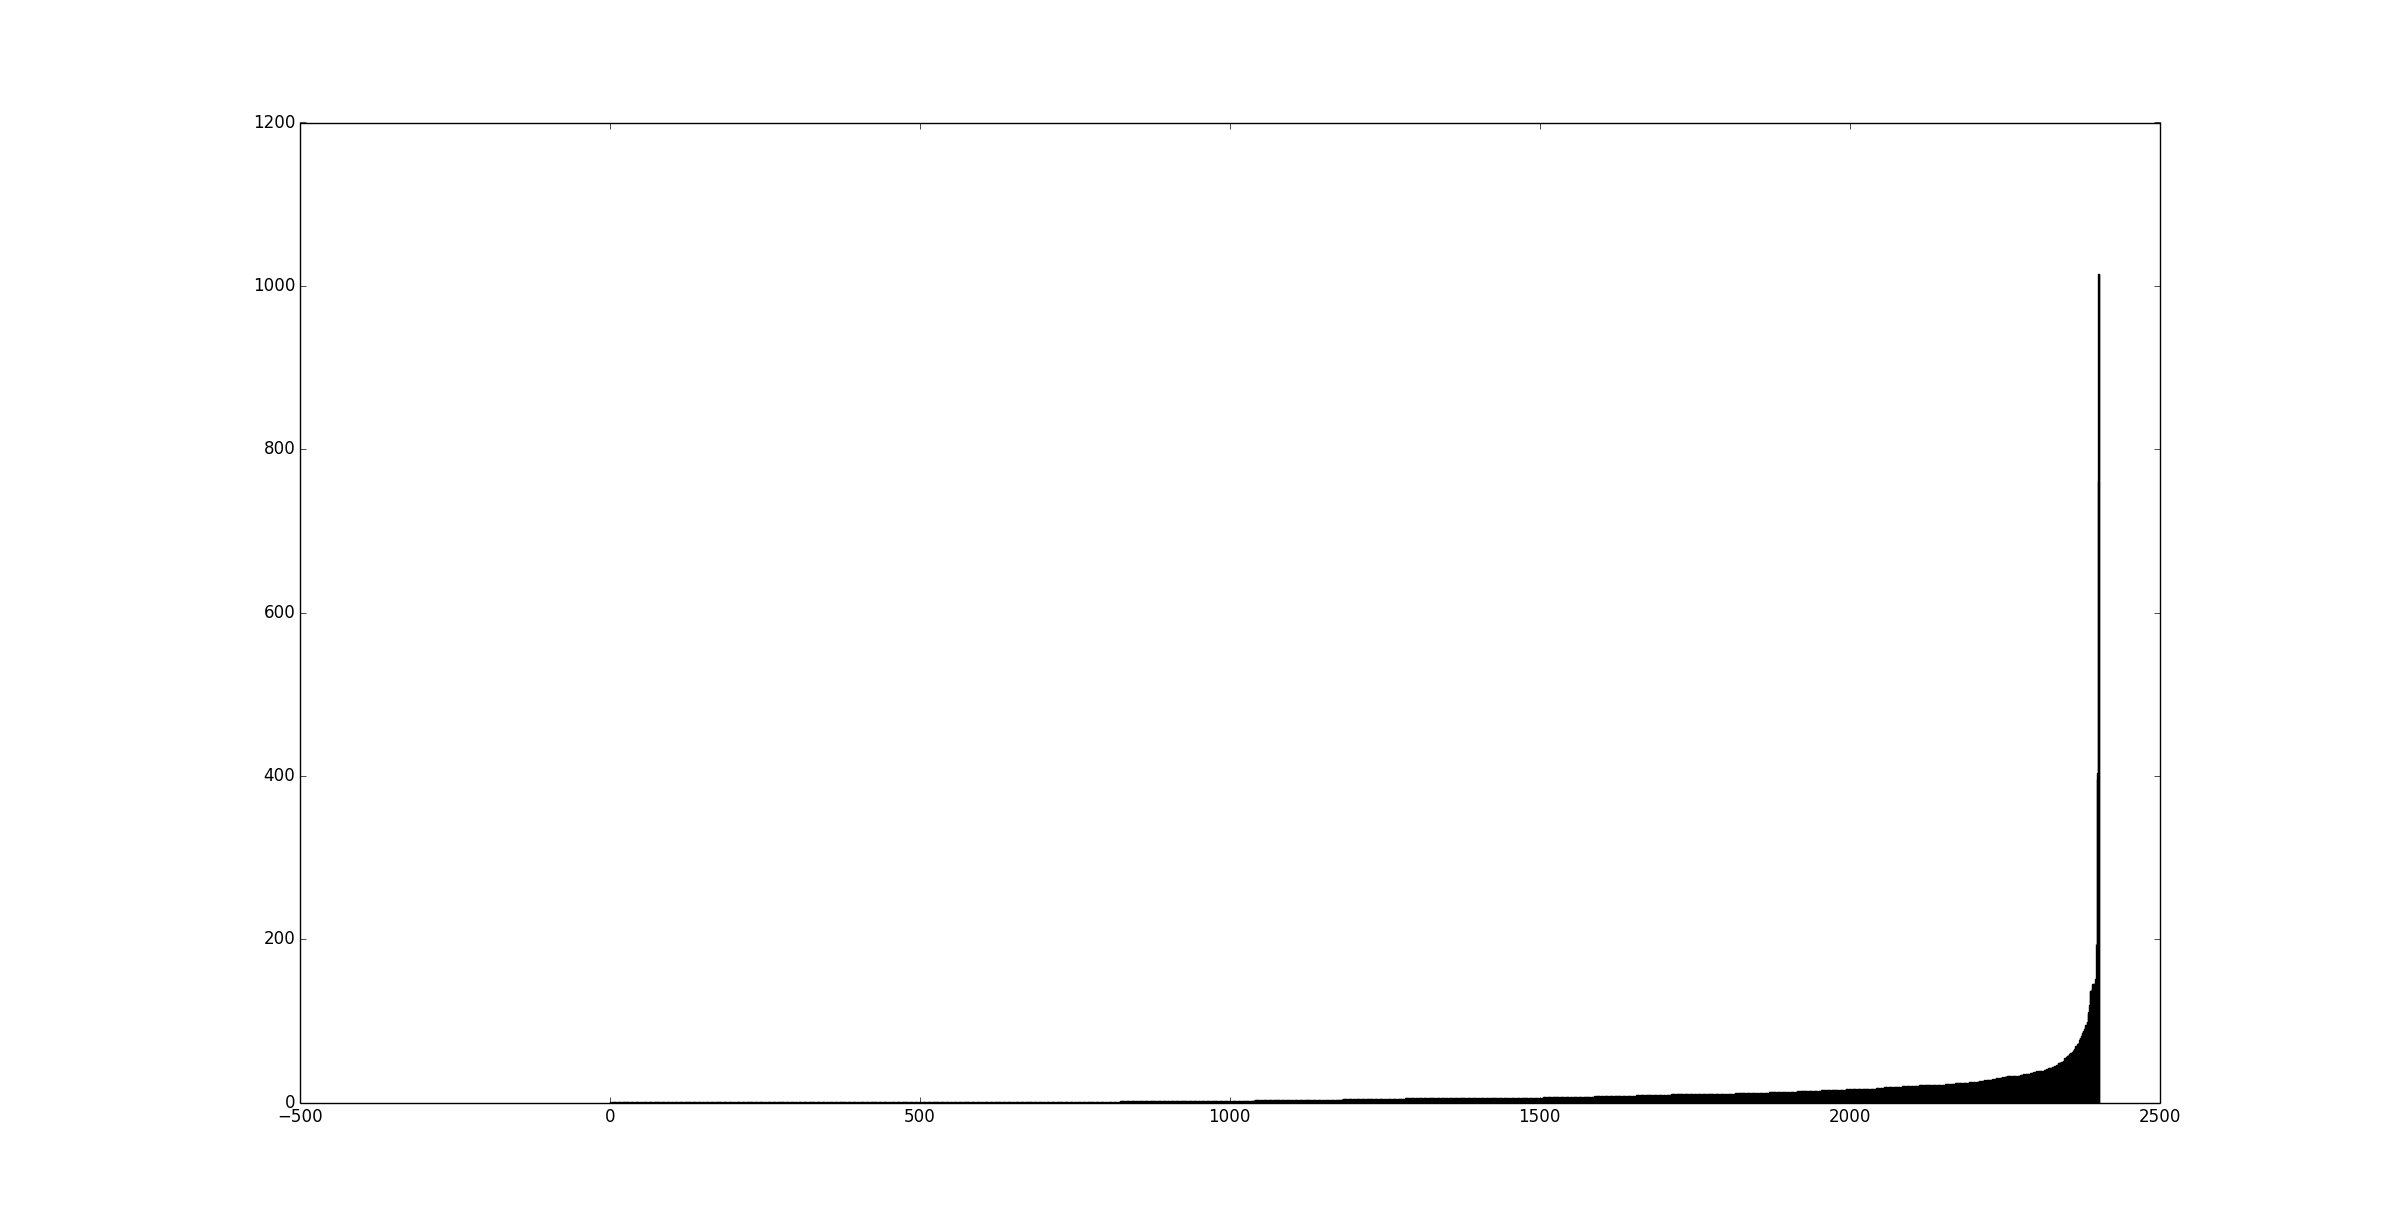
\includegraphics[width=0.5\textwidth, height=5cm]{positions}
\caption{Positions of tweet in text.}
\label{fig:positions}
\end{figure}
\improvement{Add labels to axes in graph}


\subsubsection{Percentage match}

Next, we did a percentage match with the text of the article. This was a bag-of-words check using unigrams from the tweet and the document. The order of the words in the tweet or the text did not matter. The results we got seem to suggest that a lot of significant words in the tweet are in fact present in the article. The minimum percentage match obtained was 60\%. However, since the order of the words did not matter, this result can  be traced back to the fact that tweet is based on the same topic as the document. \improvement{Calculate the number of words in common in this case}

\subsubsection{Percentage matching inside a window in the article text}

The next analysis was to check for a significant word matching inside a two or three sentence window inside the article text. We used a three sentence long window using the sentence boundary information obtained during preprocessing. After the text of the window was extracted, we performed a similar analysis as the last one, except on a smaller set of sentences. Again, the order of the unigrams didn't matter. Next, the matching percentages from all such windows in the articles were compared and the maximum out of these was considered for the highest match percentage and match position for the final results. The result from this experiment is shown in \figref{fig:percentages}. 

\begin{figure}[htbp]
\centering
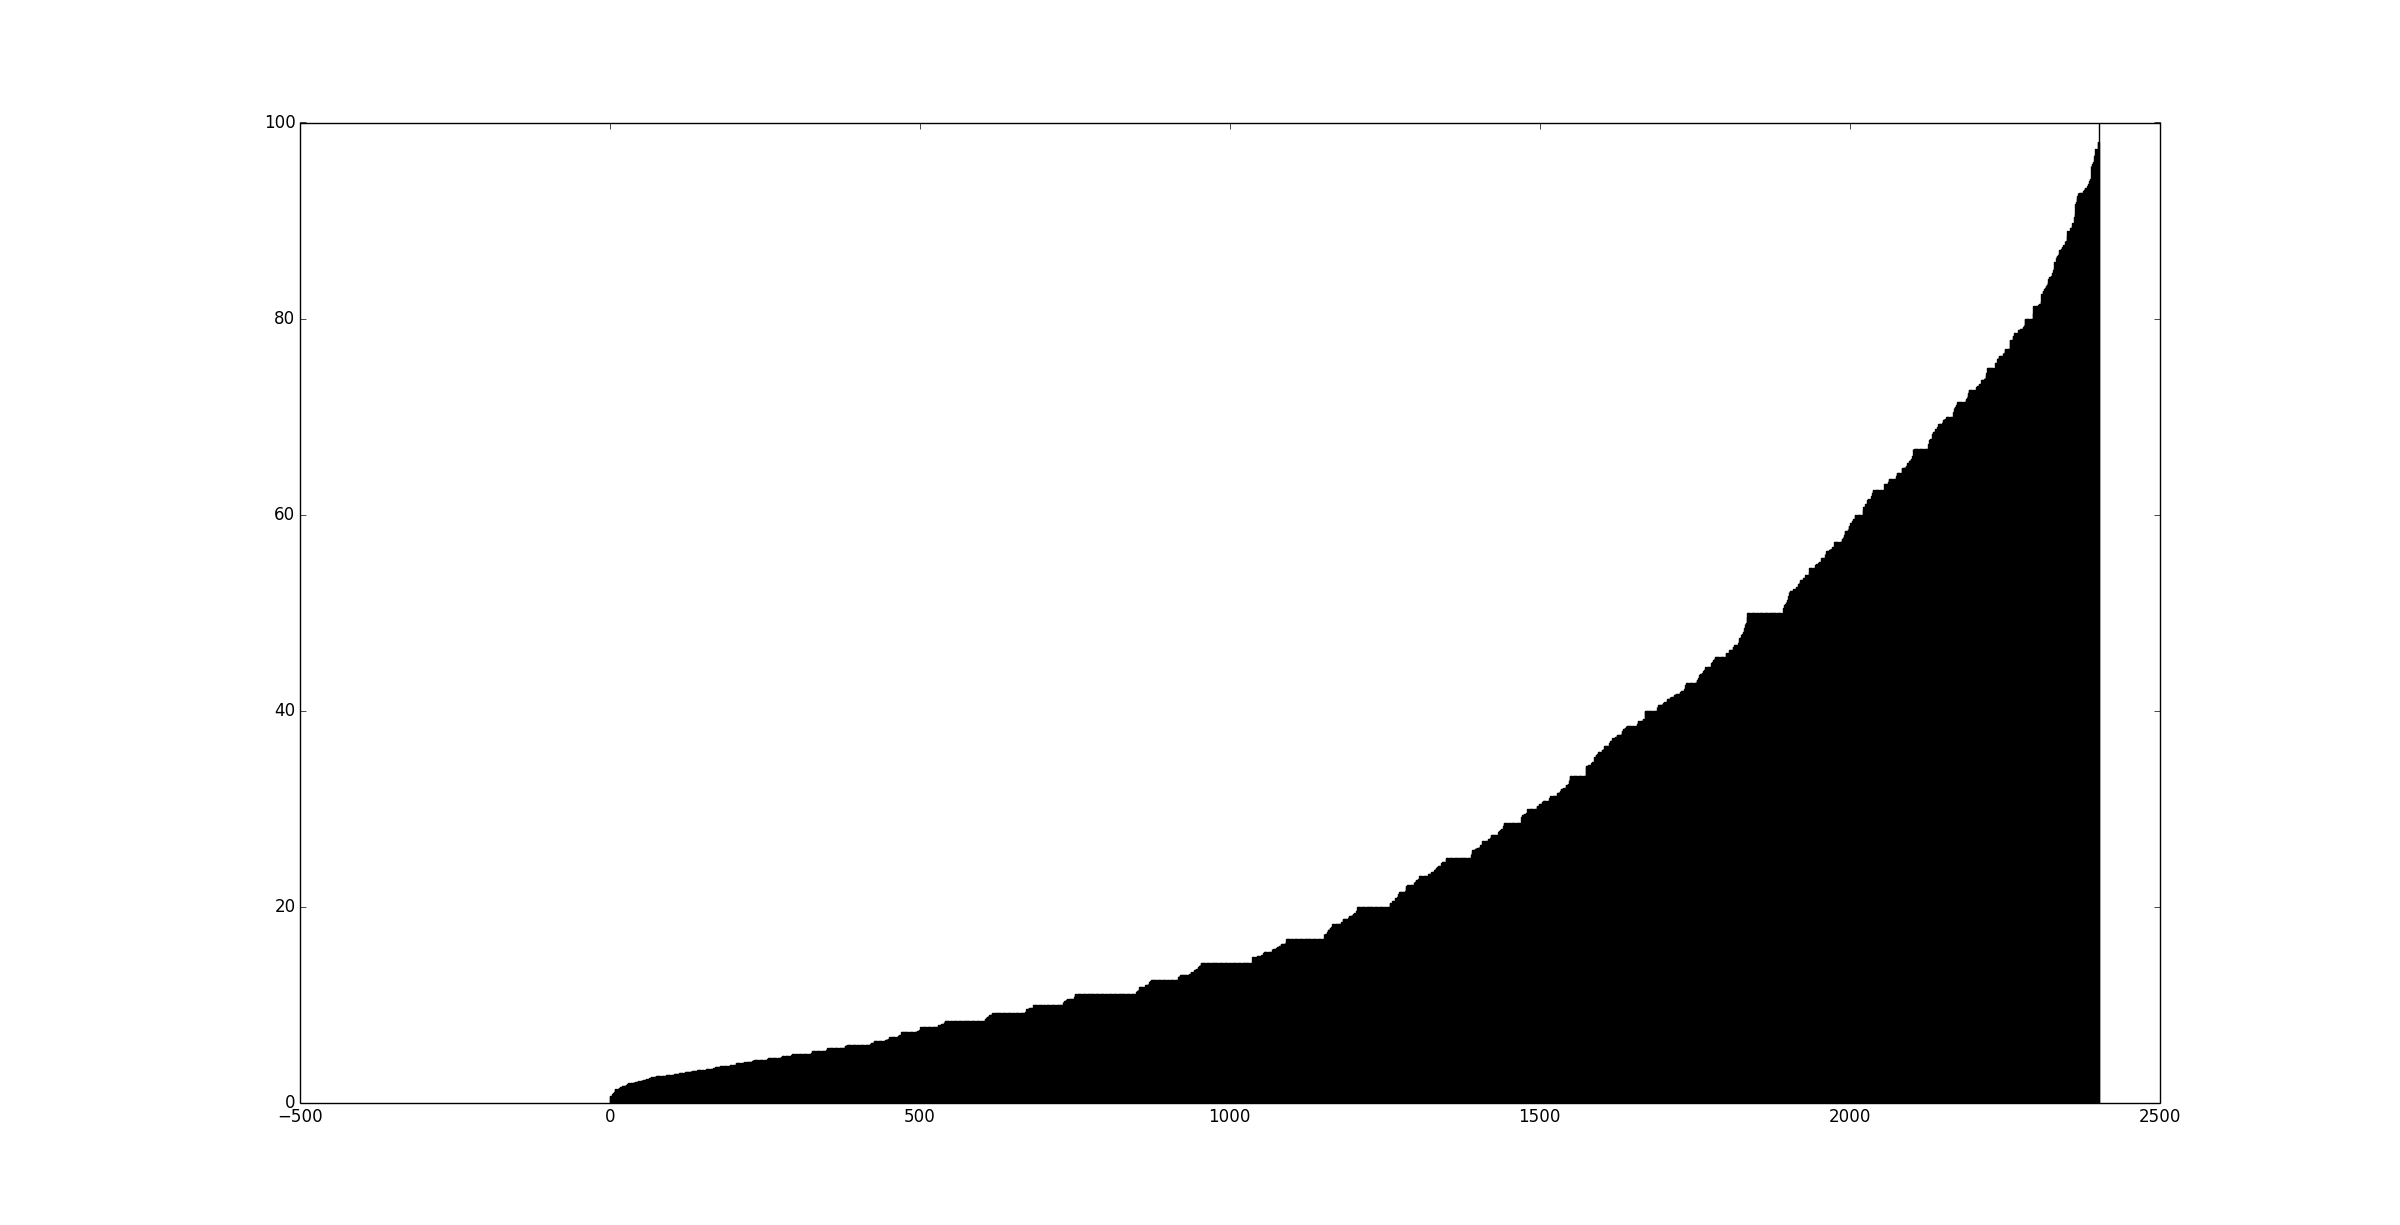
\includegraphics[width=0.5\textwidth, height=5cm]{percentages}
\caption{Percentages of common words in tweet and text.}
\label{fig:percentages}
\end{figure}
\improvement{Add labels to axes in graph}

\subsubsection{Longest Common Subsequence match inside a window for the text}

The percentage match analyses were a bag-of-words approach disregarding the order of the words inside the texts and tweets. To respect the order of the words in the sentence of the tweet, we also used the least common subsequence algorithm between the tweet text and the document text. This subsequence matching was done inside a sentence window of 5 sentences. Again, the final result for the article was the window in which the maximum percentage was recorded among all windows. The percentage match was calculated against the number of words in the tweet, as found in the least common subsequence calculated between the two texts. These numbers are shown in \figref{fig:lcs}.

\begin{figure}[htbp]
\centering
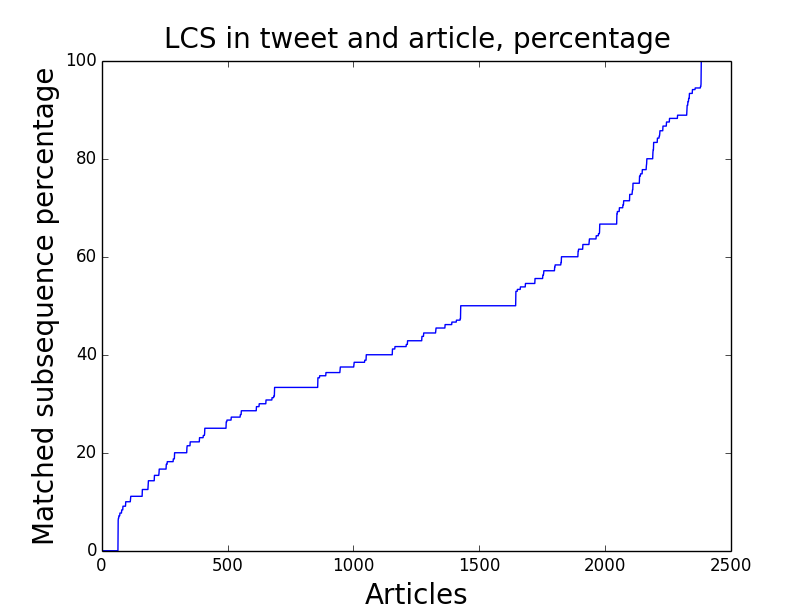
\includegraphics[width=0.5\textwidth, height=5cm]{lcs_doc}
\caption{Percentages of words matching in tweet and document text using an LCS algorithm.}
\label{fig:lcs}
\end{figure}
\improvement{Add labels to axes in graph}



\subsection{Subjectivity and Formality}
\change{should subjectivity be included?}

To achieve this, the degree of formality of the text was calculated with the help of some other studies. The formality lexicon gives was generated by \newcite{brooke2013multi} and can be used to measure formality of a given text. The lexicon consists of words and phrases and the degree of formality for their occurrence. Thus, more formal words marked on a positive scale and informal words like those occurring in colloquial language are marked on a negative scale. Using the formality and subjectivity lexicons, the degree of subjectivity and formality of each individual article was calculated. 

The degree of subjectivity returned a count per of the number of words present in the article that suggested an opinion per article. This number was normalized with the length of the article, and the degree of subjectivity was calculated per 10 words of an article. For this result, only the strong subjective entries in the lexicon were used to better differentiate between subjective and non-subjective articles.

\begin{equation}
\resizebox{.9\hsize}{!}{$formalityScore = \frac{| unigramsArticle \cap formalitySet |}{| unigramsArticle |} * 10$}
\end{equation}

The formality lexicon gave positive weights for formal expressions and negative for informal expressions. After calculating the formality weights for all articles, it was observed that they all had a total negative normalized weight, meaning a lot more informal expressions were getting matched. Hence, we used just the formal word occurrences for calculating the weight. Thus, above a certain cut-off weight, the article could be considered formal, else would be considered informal.

All the weights from both lexicons were averaged out over the articles relating to a single search term(or hashtag), and then ranked accordingly. The ranking showed that for subjectivity ranking over hashtags, films and music related hashtags are at the top, which would be the natural intuition given the nature of the topics. On the other hand, in the formality ranking, the hashtags relating to political issues had the highest formality ranking, while the hashtags for film titles, pop culture are all at the bottom. This also correlates with intuition about the topics. As a sanity check, we also looked at articles at the extreme points of the both the graphs. The texts of these articles suggested that they were consistent with the numbers.

Correlation between the rankings of hashtags given by both these experiments was calculated, and the Kendall’s tau for this was 0.09 with a p-value of 0.34. The low correlation suggests that these two ways of evaluating subjectivity and formality are independent. The p-value suggests that there is not enough evidence to prove a correlation between subjectivity and formality of an article.